\chapter{Arquitetura para compartilhamento de informações do ativo}
	
	A elaboração de uma arquitetura comum para o compartilhamento de informações do ativo é essencial para que haja consistência e interoperabilidade entre os membros da CS adotando este sistema.
	
	Esta seção tem o objetivo de apresentar detalhes da arquitetura proposta baseada em \textit{Web Services} (WS) nos modelos de uma arquitetura orientada a serviços (SOA) compatível com Componentes I4.0 para o compartilhamento de informações do ativo ao longo da CS.
	
	É apresentado também nesta seção o mapeamento dos componentes desta arquitetura dentro do eixo camadas do RAMI4.0.
	
\section{ Componentes e operações do WS }
	
	Os componentes e operações propostos para a comunicação entre ativos ao longo da \textit{Cadeia de Suprimentos} é baseada na estrutura de um WS (vide \autoref{fig:componentes-webservice}). Esta arquitetura envolve três componentes (atores) básicos: o cliente, o servidor e o repositório; e três operações: publicação, busca e interação.
	
	A interrelação entre os componentes e suas operações são mostradas na \autoref{fig:aas-wb}.
	
	\begin{figure}[htb]
		\centering
		\caption{Componentes e operações do WS.}
		\label{fig:aas-wb}
		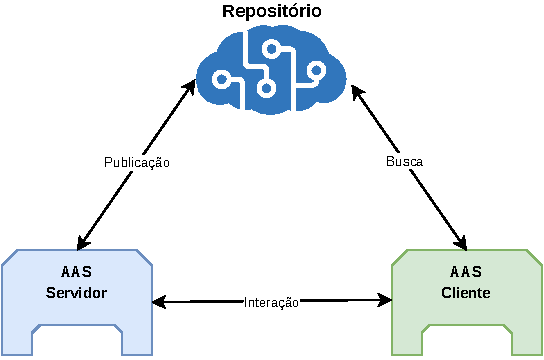
\includegraphics[width=0.7\textwidth]{aas-wb}
		\fonte{O autor.}
	\end{figure}
	
	A descrição dos serviços disponíveis nos submodelos de cada AAS devem ser publicados em um repositório comum, onde todos os AASs disponíveis no mundo conectado poderiam se tornar visíveis. A função do repositório é armazenar uma descrição dos serviços disponíveis e não o serviço em si, o serviço é fornecido pelo próprio AAS que o disponibilizou, servindo o repositório apenas como uma plataforma de descobertas de serviços.

	No modelo, cada AAS pode atuar tanto como um fornecedor de serviços, quanto um solicitante de serviços, sempre por intermédio do repositório.
	
	Quando o AAS atua como Servidor, este AAS publica a descrição de seus serviços no repositório. Quando como Cliente, o AAS busca no repositório um serviço desejado e recebe uma lista de opções de serviços com suas respectivas descrições para que possa se escolhido o mais adequado.
	
	Uma vez definido o serviço a ser consumido, o AAS Cliente e AAS Servidor estabelecem uma conexão direta, onde o cliente inicia uma interação com o servidor, utilizando os detalhes contidos na descrição do serviço para localizar, contactar e invocar o serviço.
	
	A \autoref{fig:pfs-ws} mostra o diagrama de fluxo do tipo PFS (\textit{Production Flow Schema}) inicial, envolvendo as operações de publicação, busca e interação entre os componentes.
	
	\begin{figure}[htb]
		\centering
		\caption{Diagrama PFS das operações do WS.}
		\label{fig:pfs-ws}
		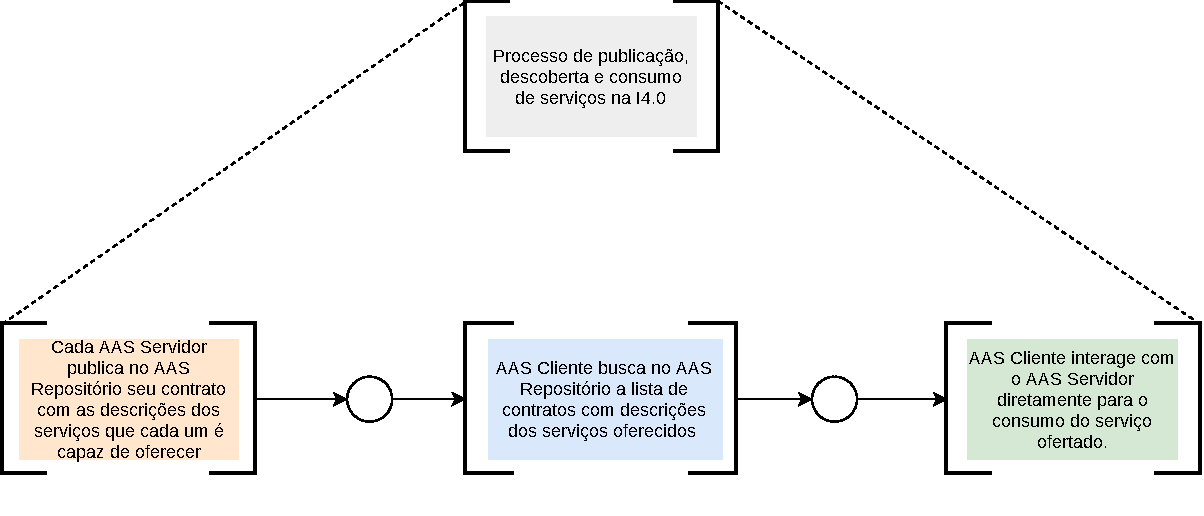
\includegraphics[width=1\textwidth]{pfs-ws}
		\fonte{O autor.}
	\end{figure}

	Os serviços fornecidos por um AAS são diversos, entretanto, neste trabalhos serão tratados com ênfase aqueles serviços que têm a função de compartilhar informações sobre o ativo que podem agregar valor ao produto ao longo de sua cadeia de valor. Ou seja, os serviços que extraem informações da MDP da AAS e as fornecem, mediante autenticação, aos partes solicitantes ao longo da cadeia de suprimentos.

\section{Estrutura do AAS e seus submodelos}

	Nesta proposta de arquitetura de WS, o conceito de Memória Digital do Produto (MDP) é inserido dentro da Indústria 4.0 com o objetivo de se agregar valor por meio da possibilidade de acesso a informações sobre o ativo entre parceiros ao longo da cadeia de valor.
	
	A MDP precisa ser integrada ao AAS para que possa ter a estrutura necessária para que seus dados sejam disponibilizados no mundo conectado da I4.0.
	
	A MDP em um AAS corresponde aos dados, ao gerenciamento desses dados e às funções básicas aplicadas em cima desses dados. A MDP contém informações referentes a cada um dos submodelos em um AAS. Cada submodelo agrega informações semelhantes relativas ao ativo.
	
	O AAS é composto pelo cabeçalho (\textit{header}) e o corpo (\textit{body}).
	
	O cabeçalho têm a função de providenciar informações públicas sobre o ativo que o identifiquem minimamente e que forneçam uma descrição sobre seus serviços oferecidos. Contém informações que podem ser acessadas sem a necessidade de autenticação, como, por exemplo, seu identificador único universal (UUID - \textit{Universal Unique IDentifier}), o modelo e fabricante do ativo. O cabeçalho contém também a descrição dos serviços fornecidos por seus submodelos. A descrição dos serviços é enviada ao repositório ou pode ser também consultada diretamente pelo AAS solicitante.
	
	A descrição de cada serviço em um cabeçalho de AAS deve necessariamente conter também referências ao AAS fornecedor, ou seja, \textit{links} e identificações que permitam o cliente localizar, contactar e invocar o serviço ofertado.
	
	O cabeçalho não tem a função de fornecer uma ficha técnica detalhada, mas apenas uma caracterização abstrata do ativo. Dependendo da confidencialidade do ativo, o submodelo de identificação pode apenas apresentar o UUID como informação pública. Sem o UUID, o AAS se torna inacessível para qualquer uma das partes da cadeia de suprimentos.
	
	O corpo (\textit{body}) de um AAS fornece as informações e funcionalidades sensíveis sobre o ativo, que podem ser acessadas mediante autenticação. As funcionalidades dos ativos são agrupadas em forma de submodelos, que são unidades de agrupamento de funcionalidades semelhantes, como propriedades, serviços e demais regras de negócio do ativo. Já os dados relativos aos submodelos são armazenadas e gerenciadas pela MDP, que também está localizada no corpo do AAS.
	
	O corpo do AAS representam a carga útil (\textit{payload}) do AAS, pois é a porção de informação que é de fato relevante para o cliente que consumirá os serviços ofertados.
	
	A estrutura proposta de um AAS compatível com WSs é apresentada na \autoref{fig:estrutura-aas}.
	
	\begin{figure}[htb]
		\centering
		\caption{Estrutura do AAS com seus submodelos e a MDP.}
		\label{fig:estrutura-aas}
		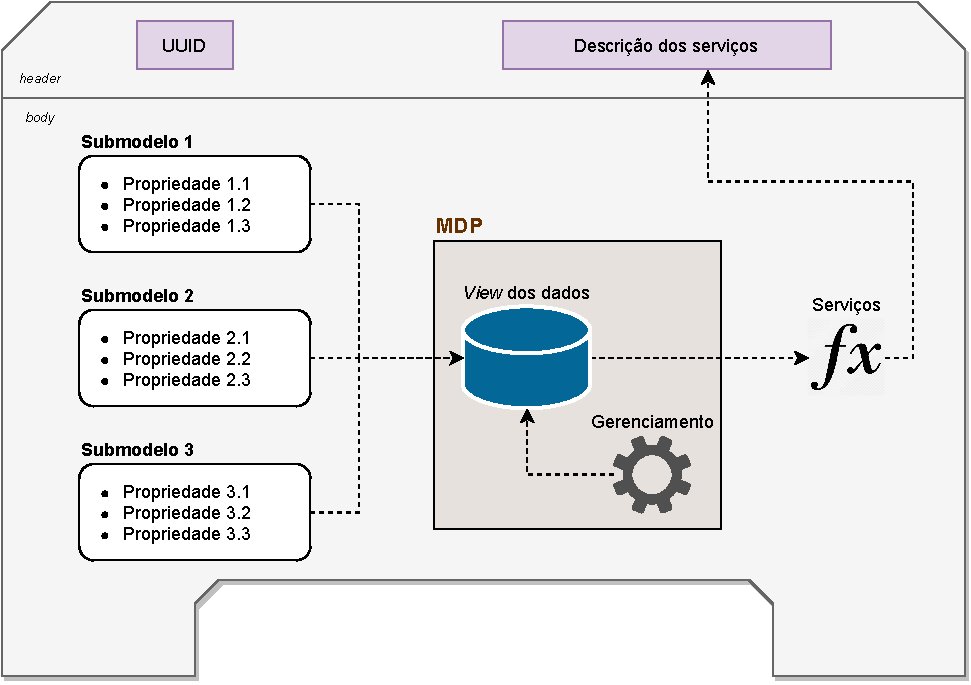
\includegraphics[width=0.7\textwidth]{estrutura-aas}
		\fonte{O autor.}
	\end{figure}

	Os dados contidos na MDP sobre submodelos, quando processados, fornecem informações sobre o ativo e agregam valor ao mesmo. Além disso, novos modelos de negócio surgem sob os dados gerados pelo ativo.
	
	Neste trabalho, é dado enfoque aos submodelos que oferecem serviços de consulta de dados a qualquer uma das partes ao longo da cadeia de suprimentos. Alguns exemplos desse tipo de submodelo podem incluir: a ficha técnica detalhada do ativo, submodelos de histórico de leitura de sensores, histórico de geolocalização do ativo, histórico de padrão de uso, etc.		

	
\section{O repositório e a descoberta de AAS's}
	
	Os submodelos \textbf{Identificação} e \textbf{Referências} são a forma primária para a identificação e acesso a um AAS, pois estes submodelos possuem o UUID do AAS e as referências para o acesso dos demais submodelos do AAS.
	
	Para que um AAS seja acessível pelas demais partes da cadeia de suprimentos, os submodelos Identificação e Referências devem estar disponíveis em uma lista pública que contém o submodelo de identificação de todos os AAS disponíveis, esta lista pública é definida como Repositório.
	
	O repositório, além de uma cópia do submodelo de identificação de cada AAS, possui também uma cópia das referências para os demais submodelos de cada AAS, conforme ilustrado na \autoref{fig:repositorio}.

	\begin{figure}[htb]
		\centering
		\caption{Repositório com referências aos AAS's.}
		\label{fig:repositorio}
		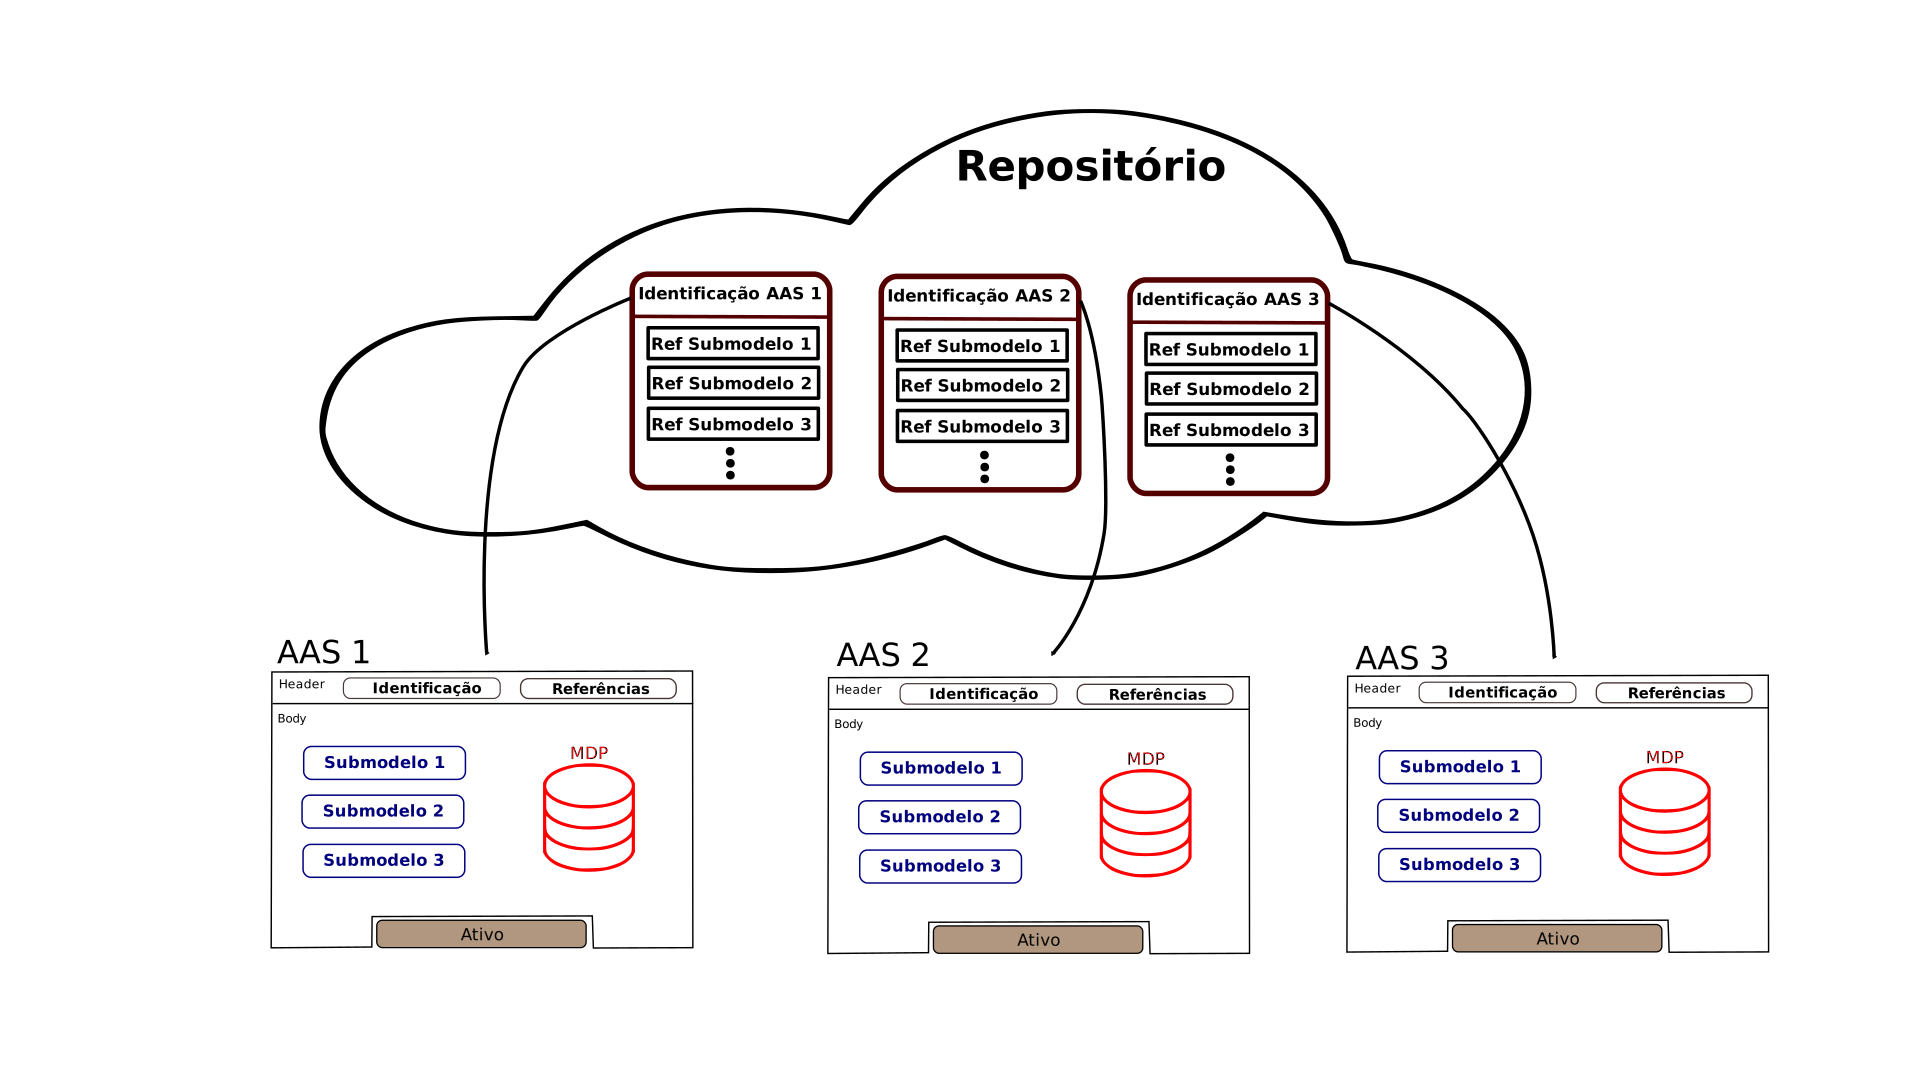
\includegraphics[width=1\textwidth]{repositorio}
		\fonte{O autor.}
	\end{figure}
	
	O repositório sob contexto da I4.0 é um \textit{web service}, ou seja, um serviço oferecido de um dispositivo eletrônico para outro dispositivo eletrônico com a comunicação entre eles por meio da \textit{World Wide Web} (Internet).
	
	Um \textit{web service} é disponibilizado por meio de um servidor que roda o serviço, escutando e respondendo solicitações de clientes através de uma determinada porta ou rede. Os clientes, por sua vez, consomem o serviço disponibilizado pelo servidor por meio de solicitações.
	
	Para o fornecimento e consumo de \textit{web services} entre cliente e servidor, diversos protocolos de comunicação podem ser utilizados na camada de aplicação do modelo padrão TCP/IP. O protocolo de comunicação para a adoção REST mais difundido na atualidade é o HTTP \cite{gruner2016restful}, porém alguns outros ainda operam, como o MQTT, que está presente principalmente na área de automação residencial e IoT \cite{yokotani2016mqtt}.
	
\section{Os quatro elos no compartilhamento de informações na CS}
	
	O modelo estrutural proposto envolve quatro componentes básicos: o AAS, a MDP, o repositório e o cliente. A \autoref{fig:4-elos} mostra as conexões entre os quatro elos, onde cada seta representa o fluxo de informações direcional. A interrelação entre as partes envolvendo o servidor REST é detalhada no Capítulo \ref{comunicacao-CS}.
	
	\begin{figure}[htb]
		\centering
		\caption{Repositório com referências aos AASs.}
		\label{fig:4-elos}
		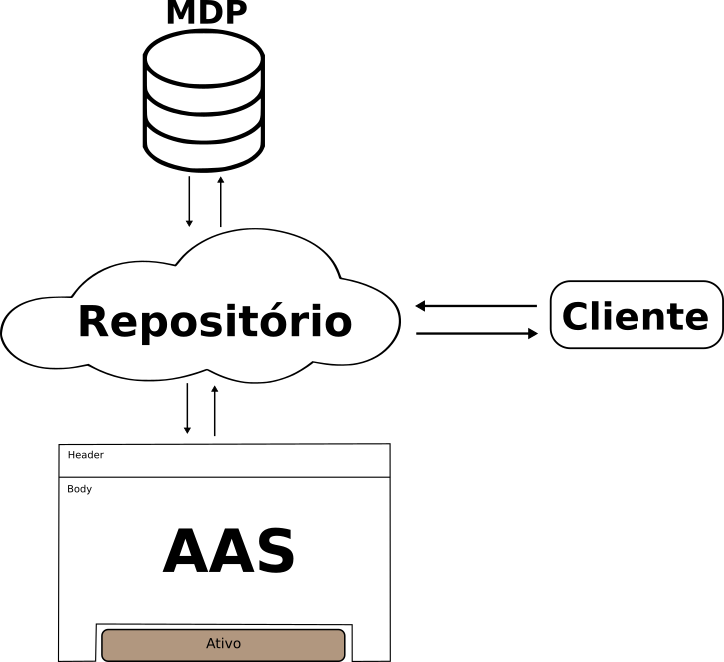
\includegraphics[width=0.8\textwidth]{4-elos}
		\fonte{O autor.}
	\end{figure}
	
	A MDP é representada neste modelo fora do AAS exclusivamente por fins didáticos. A MDP é parte do AAS. A MDP, entretanto, não estará necessariamente armazenada no escopo físico da empresa, mas oferecida em uma plataforma de serviços de computação em nuvem mais adequada para o armazenamento de grandes quantidades de dados, assim como para uma alta capacidade de requisições.
	
	Os elos necessários para o modelo estrutural de acesso a informações pelas partes da cadeia de suprimentos são detalhados na \autoref{tab:4-elos}.
	
	\begin{table}[htb]
		\centering
		\caption{Os quatro elos do modelo estrutural de acesso de informações.}
		\label{tab:4-elos}
		\begin{tabular}{lp{12cm}}
			\hline
			\rowcolor[HTML]{F0F0F0} 
			{\color[HTML]{000000} \textbf{Componente}} 
			& {\color[HTML]{000000} \textbf{Descrição}} \\ \hline
			\rowcolor[HTML]{FFFFFF} 
			{\color[HTML]{000000} AAS}         
			& {\color[HTML]{000000} O AAS é a conexão direta com o ativo, o AAS extrai e disponibiliza informações sobre o ativo. Cada submodelo do AAS representa um conjunto de informações semelhantes e suas respectivas funções de agregação.} \\
			\rowcolor[HTML]{F7F7F7} 
			{\color[HTML]{000000} Cliente}     
			& {\color[HTML]{000000} O cliente é a parte que irá consumir as informações disponibilizadas pelo AAS. O cliente representa cada uma das partes da cadeia de suprimentos, ou seja, o fabricante, o distribuidor, o consumidor, etc. }  \\
			\rowcolor[HTML]{FFFFFF} 
			{\color[HTML]{000000} Repositório}
			& {\color[HTML]{000000} O repositório é o \textit{web service} RESTful que faz a interface entre a MDP e o Cliente, ou entre a MDP e o AAS. O cliente solicita ao repositório operações de consulta ao MDP (Método GET), enquanto que o AAS solicita ao repositório operações de inserção de dados ao MDP (Método POST)}        \\
			\rowcolor[HTML]{F7F7F7} 
			{\color[HTML]{000000} MDP}
			& {\color[HTML]{000000} A memória digital do produto é o banco de dados que armazena todas as informações históricas relativas aos submodelos do AAS. A MDP não precisa necessariamente ser um banco de dados único, mas pode ser distribuído conforme a necessidade e tipo de dados a se armazenar.}       
		\end{tabular}
		\fonte{O autor.}
	\end{table}
	
\section{Estrutura de dados da MDP}

	Segundo \citeonline{radack2009exchangedata}, a série IEC 61360 fornece uma estrutura e um modelo de informação de dicionários sobre produtos. O conceito de tipo de produto é representado por ``classes'' e as características do produto são representadas por ``propriedades''.

	Tais propriedades são elementos de dados padronizados. As definições de tais propriedades podem ser encontradas em vários repositórios, como IEC CDD (dicionário de dados comuns) ou eCl@ss.
	
	A definição de uma propriedade associa um identificador exclusivo mundial a uma definição, que é um conjunto de atributos bem definidos. Atributos relevantes para o AAS são, entre outros, seu nome, o símbolo, a unidade de medida e uma definição textual legível para humanos da propriedade \cite{bader2019aas}.
	
	A publicação sugere formatos de transferência e armazenamento de dados. É especificado o UML (modelo neutro) e esquemas em XML e JSON, assim como mapeamentos para OPC UA, AutomationML e o \textit{Resource Description Framework} (RDF) \cite{plattform2019detailsaas}.
	
	A estrutura proposta usa o padrão de troca de dados JSON, que utiliza texto legível a humanos, no formato atributo-valor (natureza auto-descritiva). O um modelo de transmissão de informações no formato JSON é muito usado em \textit{web services} que usa transferência de estado representacional (REST) e aplicações AJAX, substituindo o uso do XML.
	
	A estrutura de armazenamento proposta usa banco de dados orientado a documentos que usa documento em formato JSON com esquemas pré-definidos.
	
	A \autoref{fig:json} mostra um exemplo de estruturação de dados para troca e armazenamento de informações em JSON.
	
	\begin{figure}[htb]
		\centering
		\caption{Formato de intercâmbio de informações da MDP em JSON.}
		\label{fig:json}
		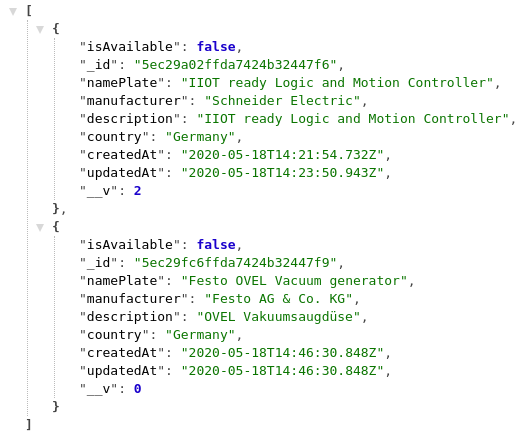
\includegraphics[width=0.8\textwidth]{json}
		\fonte{O autor.}
  \end{figure}
  

\section{Acesso à MDP pelo AAS e Cliente}
	\label{comunicacao-CS}
	
	O acesso à MDP pelo AAS a fins de escrita e pelo Cliente a fins de leitura é realizado por meio de uma API REST. No contexto na I4.0, esta API Rest é denominada ``Repositório'' e funciona como uma interface para acesso às funcionalidades do banco de dados da MDP, tais como operações CRUD (criação, leitura, atualização e exclusão).
	
	Além das operações de manipulação da MDP, o repositório serve como uma plataforma de descoberta de AAS's disponíveis, uma vez que ele contém os UUIDs de todos os AAS cadastrados.
	
\subsection{A comunicação AAS - MDP}
	
	A comunicação entre o AAS e a MDP pode ser dividida em cinco etapas:
	
	\begin{enumerate}
		\item O AAS envia ao repositório uma solicitação de inserção de dados sobre o ativo.
		\item O repositório recebe a solicitação de inserção, valida os dados, checa autenticação e envia uma soliciação de inserção de dados à MDP.
		\item A MDP processa as informações e insere em sua estrutura os novos dados.
		\item A MDP retorna uma confirmação de inserção dos dados ao repositório.
		\item O Repositório retorna ao AAS o \textit{status} da solicitação inserção de dados conforme convenções do protocolo HTTP.
	\end{enumerate}
	
	A comunicação AAS-MDP é ilustrada na \autoref{fig:aas-mdp}.
	
	\begin{figure}[htb]
		\centering
		\caption{Comunicação AAS-MDP.}
		\label{fig:aas-mdp}
		\includegraphics[width=0.8\textwidth]{aas-mdp}
		\fonte{O autor.}
	\end{figure}

\subsection{A comunicação Cliente - MDP}
	
	A comunicação entre o Cliente e a MDP, assim como a comunicação AAS-MDP, pode ser dividida em cinco etapas semelhantes:
	
	\begin{enumerate}
		\item O Cliente membro da cadeia de suprimento envia ao repositório uma solicitação de consulta de dados sobre o ativo.
		\item O repositório recebe a solicitação de consulta, checa autenticações necessárias e envia uma soliciação de consulta à MDP.
		\item A MDP processa as informações solicitadas através de uma consulta do tipo SELECT.
		\item A MDP retorna os dados solicitados ao repositório com uma confirmação de consulta executada com sucesso.
		\item O Repositório retorna ao Cliente os dados solicitados juntamento com o \textit{status} da solicitação de consulta conforme convenções do protocolo HTTP.
	\end{enumerate}
	
	A comunicação Cliente-MDP é ilustrada na \autoref{fig:cliente-mdp}.
	
	\begin{figure}[htb]
		\centering
		\caption{Comunicação Cliente-MDP.}
		\label{fig:cliente-mdp}
		\includegraphics[width=0.8\textwidth]{cliente-mdp}
		\fonte{O autor.}
	\end{figure}
	
	
\subsection{Interação AAS-MDP-Cliente}
	
	A interação AAS-MDP-Cliente é basicamente uma operação simultânea assíncrona da comunicação AAS-MDP e a comunicação Cliente-MDP.
	
	Nesta interação, diversos AAS's e diversos clientes podem fazer solicitações independentes ao repositório de operações CRUD.
	
	A \autoref{fig:aas-mdp-cliente} ilustra interações simultâneas entre o cliente ou o AAS com o repositório para solicitações de leitura e solicitações de escrita na MDP, respectivamente.
	
	\begin{figure}[htb]
		\centering
		\caption{Comunicação Cliente-MDP.}
		\label{fig:aas-mdp-cliente}
		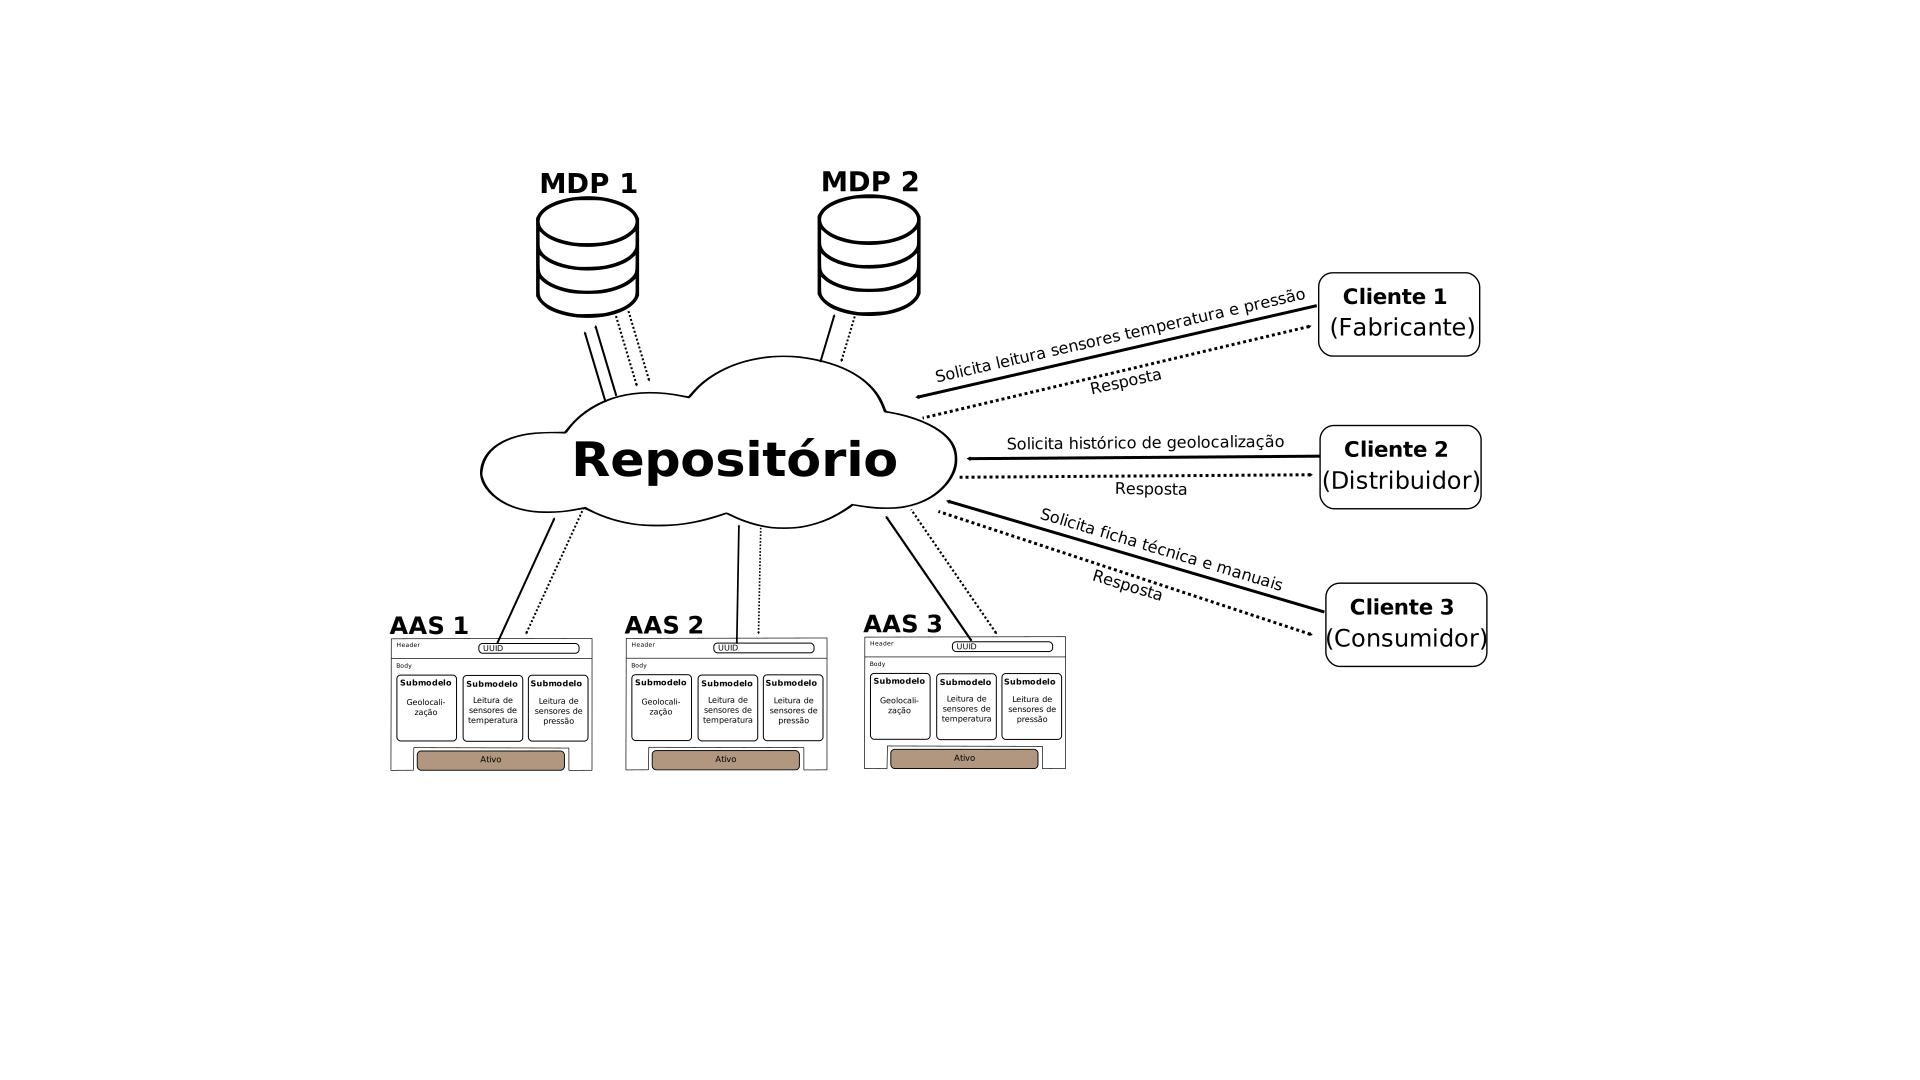
\includegraphics[width=1\textwidth]{aas-mdp-cliente}
		\fonte{O autor.}
	\end{figure}

	Cada AAS não precisa necessariamente estabelecer conexão com apenas uma MDP, diferentes submodelos de uma AAS podem ter seus dados salvos em diferentes serviços de armazenamento em nuvem, ou até mesmo em um banco de dados local na própria empresa.
	
	Cada cliente deve se autenticar junto ao repositório a fim de ser consultar a MDP. Isto significa que cada cliente não tem o acesso integral a todos os submodelos do AAS, mas somente àquele que for determinado por projeto.
	
	Na \autoref{fig:aas-mdp-cliente} são exemplificados três tipos de clientes com seus respectivos escopos de autenticação. O Cliente 1 pode acessar somente informações relativas ao submodelo de leitura de sensores de temperatura e pressão, o Cliente 2 pode acessar somente informações sobre o submodelo de geolocalização, o Cliente 3 acessa somente o submodelo de ficha técnica e manuais.
	
	\section{O MDP e as Camadas do RAMI4.0}

	Segundo \citeonline{iec2017rami}, o RAMI4.0 fornece uma visão estruturada dos principais elementos de um ativo, usando um modelo de níveis composto por três eixos. Desta forma, interrelações complexas podem ser divididas em seções menores e mais gerenciáveis, combinando os três eixos em cada ponto da vida do ativo para representar cada aspecto relevante.
	
	Desta forma, a coparticipação da MDP deve ser representada também conforme a estrutura do RAMI4.0, explicitando em que parte acontece cada interação entre AAS, MDP, Repositório e Cliente.
